\documentclass[a4paper, 12pt]{report}

\usepackage[spanish]{babel}
\usepackage[utf8]{inputenc}
\usepackage[left=4cm, right=4cm, top=4cm]{geometry}
\usepackage{textcomp}
\usepackage{booktabs}
\usepackage{amssymb}
\usepackage{bussproofs}
\usepackage{fancyhdr}
\usepackage{graphicx}
\usepackage{amsmath}
\usepackage{enumitem}


\usepackage{hyperref}
\hypersetup{
    colorlinks=true,
    linkcolor=blue,
    filecolor=magenta,
    urlcolor=cyan,
}

\pagestyle{fancy}
\lhead{Almeida, Figueroa \& Ibarra}
\chead{Tarea 3}
\rhead{\today}

\begin{document}
\begin{titlepage}
    \centering
    {\scshape\Huge Universidad Nacional Autónoma de México \par}
    \vspace{1.25cm}
    {\scshape\huge Fundamentos de Bases de Datos\par}
    \vspace{1.25cm}
    {\huge\bfseries Tarea 3: Modelo Relacional\par}
    \vspace{1.25cm}
    {\Large\textsc Almeida Rodríguez Jerónimo\par}
    \vspace{.1cm}
    {\large\texttt{418003815}\par}
    \vspace{0.25cm}
    {\Large\textsc Figueroa Sandoval Gerardo Emiliano\par}
    \vspace{.1cm}
    {\large\texttt{315241774}\par}
    \vspace{0.25cm}
    {\Large\textsc Ibarra Moreno Gisselle \par}
    \vspace{.1cm}
    {\large\texttt{315602193}\par}
    \vspace{1.5cm}
    \vfill
    \begin{figure}[hb!]
        
\includegraphics[width=.3\textwidth]
            {../logos/escudo_f-ciencias.png}\hfill
        
\includegraphics[width=.3\textwidth]
            {../logos/Escudo_UNAM.png}\hfill
    \end{figure}
\end{titlepage}

\section*{1. Preguntas de Repaso.}{
	\begin{enumerate}[label=(\alph*)]
		\item  ¿Qué es una \textbf{relación} y qué características 	
		tiene?\\
		Es un modelo de organización y gestión de bases de datos 				consistente en el almacenamiento de datos en tablas compuestas 		por filas, o tuplas, y columnas o campos.Surge como solucio´n a 		la creciente variedad de los datos que integran las data 				warehouses y podemos resumir el concepto como una colecci´on 	
		de tablas (relaciones). Estas tablas, pueden ser constru´ıdas 	
		de diversas maneras:
		\begin{itemize}
			\item Creando un conjunto de tablas iniciales y aplicar 				operaciones de normalización hasta conseguir el esquema 				más óptimo.
			\item Convertir el diagrama e-r a tablas y posteriormente 	
			aplicar también operaciones de normalizacio´n hasta 	
			conseguir el esquema óptimo.
		\end{itemize}		 
		\item  ¿Qué es un \textbf{esquema de relación}?\\
		Es el que contiene la definición de una estructura 	
		(generalmente relaciones o tablas de una base de datos), es 	
		decir, determina la identidad de la relación y qué tipo de 	
		información podrá ser almacenada dentro de ella; en otras 	
		palabras, el esquema contiene los metadatos de la relación. 	
		Todo esquema constará de:
		\begin{itemize}
			\item Nombre de la relación (su identificador).
			\item Nombre de los atributos (o campos) de la relación y 				sus dominios; el dominio de un atributo o campo define los 	
			valores permitidos para el mismo, equivalente al tipo de 	
			dato por ejemplo character, integer, date, string..
		\end{itemize}
		\item  ¿Qué es una \textbf{llave primaria}?, ¿qué es una 		
		\textbf{llave candidata}?, ¿qué es una \textbf{llave mínima}?, 		¿qué es una \textbf{super llave}?
		\begin{itemize}
			\item \textbf{Llave primaria}: Una llave primaria es un 	
			conjunto de uno o más atributos de una tabla, que tomados 	
			colectivamente nos permiten identificar un registro como 				único, es decir, en una tabla podemos saber cual es un 	
			registro en específico sólo con conocer la llave 	
			primaria.
			\item \textbf{Llave candidata}:  Una llave candidata es					el atributo o conjunto de atributos que 	
			tienen la propiedad de identificar unívocamente a una 	
			tupla dentro de la relación. Las llaves constituyen el 	
			mecanismo de direccionamiento a nivel de tuplas básico en 				un sistema relacional, es decir, es el único modo, 						garantizado por el sistema, de localizar alguna tupla 					específica.
			\item\textbf{Super llave}: Una super llave es un conjunto 				de uno o más atributos que tomados colectivamente,permiten 			identificar de forma única una entidad en el conjunto de 
			entidades.
			\item \textbf{Llave mínima}: Es equivalente a la llave 		
			candidata.
		\end{itemize}
		\item ¿Qué restricciones impone una \textbf{llave primaria} y 			una \textbf{llave foránea} al modelo de datos relacional?
		\begin{itemize}
			\item \textbf{Llave primaria}: Una tabla suele tener una 	
			columna o una combinación de columnas cuyos valores 	
			identifican de forma única cada fila de la tabla. Estas 	
			columnas se denominan claves principales de la tabla y 	
			exigen la integridad de entidad de la tabla. Debido a que 	
			las restricciones de clave principal garantizan datos 	
			únicos, con frecuencia se definen en una columna de 	
			identidad.\\
			Cuando especifica una restricción de clave principal en 	
			una tabla, Motor de base de datos exige la unicidad de los 			datos mediante la creación automática de un índice único 	
			para las columnas de clave principal. Este índice también 	
			permite un acceso rápido a los datos cuando se usa la 	
			clave principal en las consultas. Si se define una 	
			restricción de clave principal para más de una columna, 	
			puede haber valores duplicados dentro de la misma columna, 			pero cada combinación de valores de todas las columnas de 	
			la definición de la restricción de clave principal debe 	
			ser única.
			\item \textbf{Llave foránea}: Una clave externa (FK) es 	
			una columna o combinación de columnas que se usa para 	
			establecer y aplicar un vínculo entre los datos de dos 	
			tablas a fin de controlar los datos que se pueden 	
			almacenar una tabla de clave externa. En una referencia de 			clave externa, se crea un vínculo entre dos tablas cuando 	
			las columnas de una de ellas hacen referencia a las 	
			columnas de la otra que contienen el valor de clave 	
			principal. Esta columna se convierte en una clave externa 	
			para la segunda tabla.\\
			A diferencia de las restricciones de clave principal, la 	
			creación una restricción de clave externa no crea 	
			automáticamente el índice correspondiente. No obstante, la 			creación manual de un índice en una clave externa suele 				ser útil por los siguientes motivos:
			\begin{itemize}
				\item Las columnas de clave externa suelen usarse en 	
				los criterios de combinación cuando los datos de las 	
				tablas relacionadas se combinan en consultas mediante 	
				la correspondencia de la columna o columnas de la 	
				restricción de clave externa de una tabla y la columna 				o columnas de la clave única o principal de la otra. 	
				Un índice permite al Motor de base de datos buscar con 				rapidez datos relacionados en la tabla de clave 	
				externa. No obstante, no es necesario crear este 	
				índice.
				\item Los cambios en las restricciones de clave 	
				principal se comprueban con restricciones de clave 	
				externa en las tablas relacionadas.
			\end{itemize}
		\end{itemize}
		 \item Investiga cómo se traducen las \textbf{categorías} 	
		 (presentes en el \textbf{modelo E/R}) al \textbf{modelo 	
		 relacional}. Proporciona un ejemplo.
		 \begin{itemize}
		 	\item \textbf{Entidad a Tabla}:Los identificadores 	
		 	conforman la clave primaria, los atributos requeridos las 	
		 	definiciones de valor no nulo (columnas que no admiten 	
		 	nulos), en general cada atributo será una columna de esa
		 	tabla.
		 	\begin{itemize}
		 		\item \textbf{Identificador compuesto}: Todo aquello 	
		 		que aparezca subrayado entrará a formar parte de la 	
		 		clave primaria, es el identificador, compuesto o no, 	
		 		de la entidad. Dicho de otra forma, NO terminan siendo 				dos claves candidatas distintas.
		 		\item \textbf{PERDIDAS}: Los atributos compuestos es 	
		 		una de esas pérdidas semánticas, aunque poco 	
		 		importante. Al final, simplemente tendremos una 	
		 		columna por cada atributo simple.\\
		 		Los atributos multivaluados no tienen una traducción 	
		 		directa, hay que tomar alguna decisión de diseño y 	
		 		generar alguna tabla adicional. 
			\end{itemize}
			\item \textbf{Relaciones 1:N a Tabla}: En cuanto a las 	
			correspondencias entre clases, las relaciones entre 	
			entidades, todo está muy ligado a lo que se está viendo 	
			relativo al modelo relacional. Evidentemente, si el E-R 	
			muestra una relación 1:N su traducción a tablas será una 	
			relación 1:N... en tablas.\\
			En cualquier caso, las relaciones en E-R, las 	
			cardinalidades y los triángulos, se traducen a una clave 	
			ajena, es decir, una (o varias, depende de la clave 	
			primaria a la que apunte) columnas adicional  que es clave 			ajena. Siempre se trata de columnas que hay que añadir a 	
			la tabla resultado.\\
 			Por eso no hace falta especificarlas en E-R, lo importante 			es el hecho que representa, que hay una relación entre el 				concepto A y el B. En E-R se hace dibujando los símbolos 				correspondientes; en MR añadiendo claves ajenas. 
 			\begin{itemize}
 				\item \textbf{Restricción de existencia }: En el caso 	
 				de las relaciones uno a muchos (1:N) se trata de 	
 				colocar una clave ajena en la tabla que sufre las 	
 				restricciones.
 				\item \textbf{Doble restricción de existencia}:Termina 				casi siempre cambiando las pautas de diseño para 		
 				transformarla, ya, en una única entidad). No obstante, 				teniendo cierto sentido representarla así en E-R, hay 	
 				que tener claro que su traducción, la verdaderamente 	
 				eficiente desde un punto de vista estructural, es una 	
 				única tabla sin claves ajenas pero con una clave 	
 				primaria y otra alternativa. 
 			\end{itemize}
 			\item \textbf{Relaciones N:M a Tabla}: Lo mejor es una 	
 			tercera tabla con 2 claves ajenas, pero ahora la clave 	
 			primaria se compone con esas dos claves ajenas.\\
			Debe hacerse notar que, mientras en E-R es posible definir 			restricciones de existencia sobre esta relación, en MR 	
			necesariamente ha de considerarse una pérdida semántica si 			queremos que nuestra representación, este conjunto de 	
			tablas, se comporte realmente como una N:M. 
			\item \textbf{Relaciones a Tabla Generalizaciones}: En el 	
			caso de las generalizaciones, aparte de la tabla con los 	
			datos comunes a todas las subclases, necesitamos una tabla 			por cada categoría que nos encontremos en el E-R. Esas 	
			tablas comparten el hecho de que definen una clave ajena 	
			que es exactamente la clave primaria. Aparte, se definirán 			tantas columnas como atributos propios tenga la entidad.  
		 \end{itemize}
		 \begin{center}
		 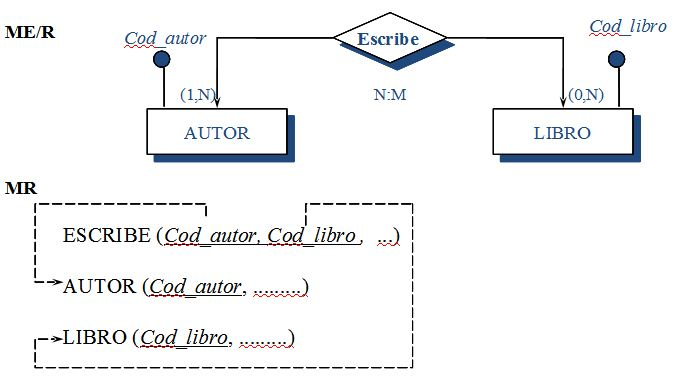
\includegraphics[scale= 0.7]{img/Ejemplo.jpg}
		 \end{center}	 
	\end{enumerate}
}

\section*{2. Modelo Relacional.}{
}

\section*{3. Lectura.}{
\begin{enumerate}
\item[1.]{\textbf{Regla de Información: } \\
    \textit{Toda la Información en la base de datos está representada de una
    manera única, cómo valores en tablas.}\\
    En general, toda la información se guarda en tablas.
}
\item[2.]{\textbf{Regla del Acceso Garantizado: }\\
    \textit{Está garantizado que cada dato (valor atómico) pueda ser accedido
    lógicamente por medio de una combinación de nombre de tabla, valor de la
    llave primaria y el nombre de la columna.}\\
    Esta regla lo que busca es garantizar el acceso a la información de manera
    única por medio de un conjunto de ``coordenadas'' que, basadas en el nombre
    de la tabla, la llave primaria y el nombre de la columna, permite que cada
    dato pueda recuperarse de manera única.
}
\item[3.]{\textbf{Tratamiento Sistematico de los Valores 'NULL': }\\\textit{
    Los valores NULL son usados en SMBDR para representar informanción faltante
    o desconocida de una manera sistemática, independientemente del tipo de dato.
    Son distintos del caracter de cadena vacía, de caracteres blancos y de
    cualquier número.}\\
    Implementa el uso de valores NULL, que en general significan que el valor
    es desconocido. Usualmente se trata cómo operar el vacío ($\O$) en teoría de
    conjuntos: cualquier cosa operada con NULL devuelve NULL; aunque en algunos
    casos, si se intenta concatenar con una cadena, devuelve la nueva cadena.
}
\item[4.]{\textbf{Catálogo Dinámico en Línea Basado en el Modelo Relacional:}\\
    \textit{En el nivel lógico, la descripción de la base de datos está
    representada al mismo nivel que los datos ordinarios. De esta manera, los
    usuarios autorizados pueden usar el mismo lenguaje relacional que se usa
    para datos regulares.}\\
    En general requiere que el sistema sea autodescriptivo.
}
\item[5.]{\textbf{Regla del Sublenguaje de Datos Comprensivos:}\\
    \textit{
    Un sistema relacional puede soprtar varios lenguajes de programación y modos
    de uso terminal, pero al menos uno de ellos debe tener expresiones que sean
    expresables por medio de una sitáxis bien definida y puede soportar lo
    siguiente:}
    \begin{itemize}
        \item\textit{{Definición de datos.}}
        \item\textit{{Visibilización de la definición.}}
        \item\textit{{Manipulación de datos}}
        \item\textit{{Restricciones de integridad.}}
        \item\textit{{Autorizaciones.}}
        \item\textit{{Bordes de transacciones (inicio, commit, etc.).}}
    \end{itemize}
    Esta restricción requiere que el sistema tenga un lenguaje que pueda manipular
    (recuperar, insertar, borrar, etc.) la información dentro de la base de datos.
}
\item[6.]{\textbf{Regla de la vista actualizada:}\\
    \textit{Todas las vistas que se pueden actualizar las puede actualizar el
    sistema.}\\
    Esta regla requiere que los distintos usuarios puedan ver la estructura de
    las bases de datos.\\
    Es una de las reglas más difíciles de implementar, de tal manera que ningún
    SMBD la satisface completamente. En SQL Server, las vistas se actualizan
    solamente si no se actualiza más de una tabla en un momento dado.
}
\item[7.]{\textbf{Insert, Delete y Actualizar a Alto Nivel:}\\
    \textit{La abilidad de manejar una relación base o derivada cómo un único
    operando no solo al recuperar la información sino también para insertar,
    borrar y actualizar información.}\\
    Esta regla establece que la información debe ser manipulada cómo conjuntos,
    lo que ayuda a garantizar la consistencia de la base de datos.
}
\item[8.]{\textbf{Independencia Física de Datos:}\\\textit{
    Los programas de aplicación y actividades terminales se mantienen funcinando
    cuándo hay cambios en la representación de almacenamiento o métodos de
    acceso.}\\
    El objetivo es que el almacenamiento de los datos sea independiente del
    programa que los requiere pero asegurando que pueden ser accedidos de la
    misma manera.
}
\item[9.]{\textbf{Independencia Lógica de Datos:}\\\textit{
    Los programas de aplicación y actividades terminales se mantienen lógicamente
    funcionales cambios que preserven la información se haga en alguna tabla.}\\
    Establece que la manera específica de acceder a la base de datos no debe afectar
    la abilidad del usuario de manipular los datos.
}
\item[10.]{\textbf{Independencia de Integridad:}\\\textit{
    Las restricciones de integridad específicas de de una base relacional deben
    poder ser definidas en el lenguaje de el lenguaje relacional y deben poder
    ser almacenadas en el catálogo, no en los programas de aplicación. Protege la
    información de datos inválidos.}\\
    Este regla intenta mantener la integridad de la base de datos, particularmente
    en lo relacionado a todo aquello que se puede acceder por medio de una llave
    primaria o foranea.
}
\item[11.]{\textbf{Independencia de Distribución:}\\\textit{
    El lenguaje del SMBD debe permitir que los programas de aplicación y actividades
    terminales permanezcan lógicamente funcionales y accesibles ya sea que los datos
    estén físicamente cnetralizados o distribuidos.}\\
    El objetivo de esta regla es mantener una base de datos ``unificada'' aunque
    la información se encuentre físicamente repartida en dispositivos diferentes.
    Esto significa que a pesar de estar separada cumple (idealmente) con las
    propiedades que una base de dato debe cumplir.
}
\item[12.]{\textbf{Regla de No-Subversión:}\\\textit{
    Si un sistema relacional permite el uso de slgún lengiaje de programación de
    un nivel más bajo, este lenguaje no puede ser usado para traspasar las reglas
    de integridad y restricciones establecidas por el lenguaje relacional.}\\
    El objetivo es que no haya manera de acceder a la información fuera de la
    establecida por el SMBDR. Esto con el objetivo de mantener la integridad
    del sistema.\\\\
}
La importancia de estas reglas radica en mantener un sistema que a lo largo de su
ejecución sea capaz de mantener consistencia en la información que almacena además
de de establecer una manera de manipular y acceder a la información de manera
consistente y confiable.\\
Cómo establece el artículo, tanto la regla 6 cómo la 12 no se pueden cumplir
enteramente por los SMDBR actuales.

\end{enumerate}
}




\end{document}
